\section{Equações Básicas}
Expressões gerais para coeficientes de rigidez e ações de engastamento e outras grandezas importantes para a formulação do método dos deslocamentos podem ser obtidas a partir de equações de equilíbrio e condições de compatibilidade relacionadas ao elemento estrutural. Considerando-se o elemento de pórtico plano mostrado na Fig \ref{fig:el-portico-plano}, resulta:

\begin{figure}[!htbp]
	\centering
	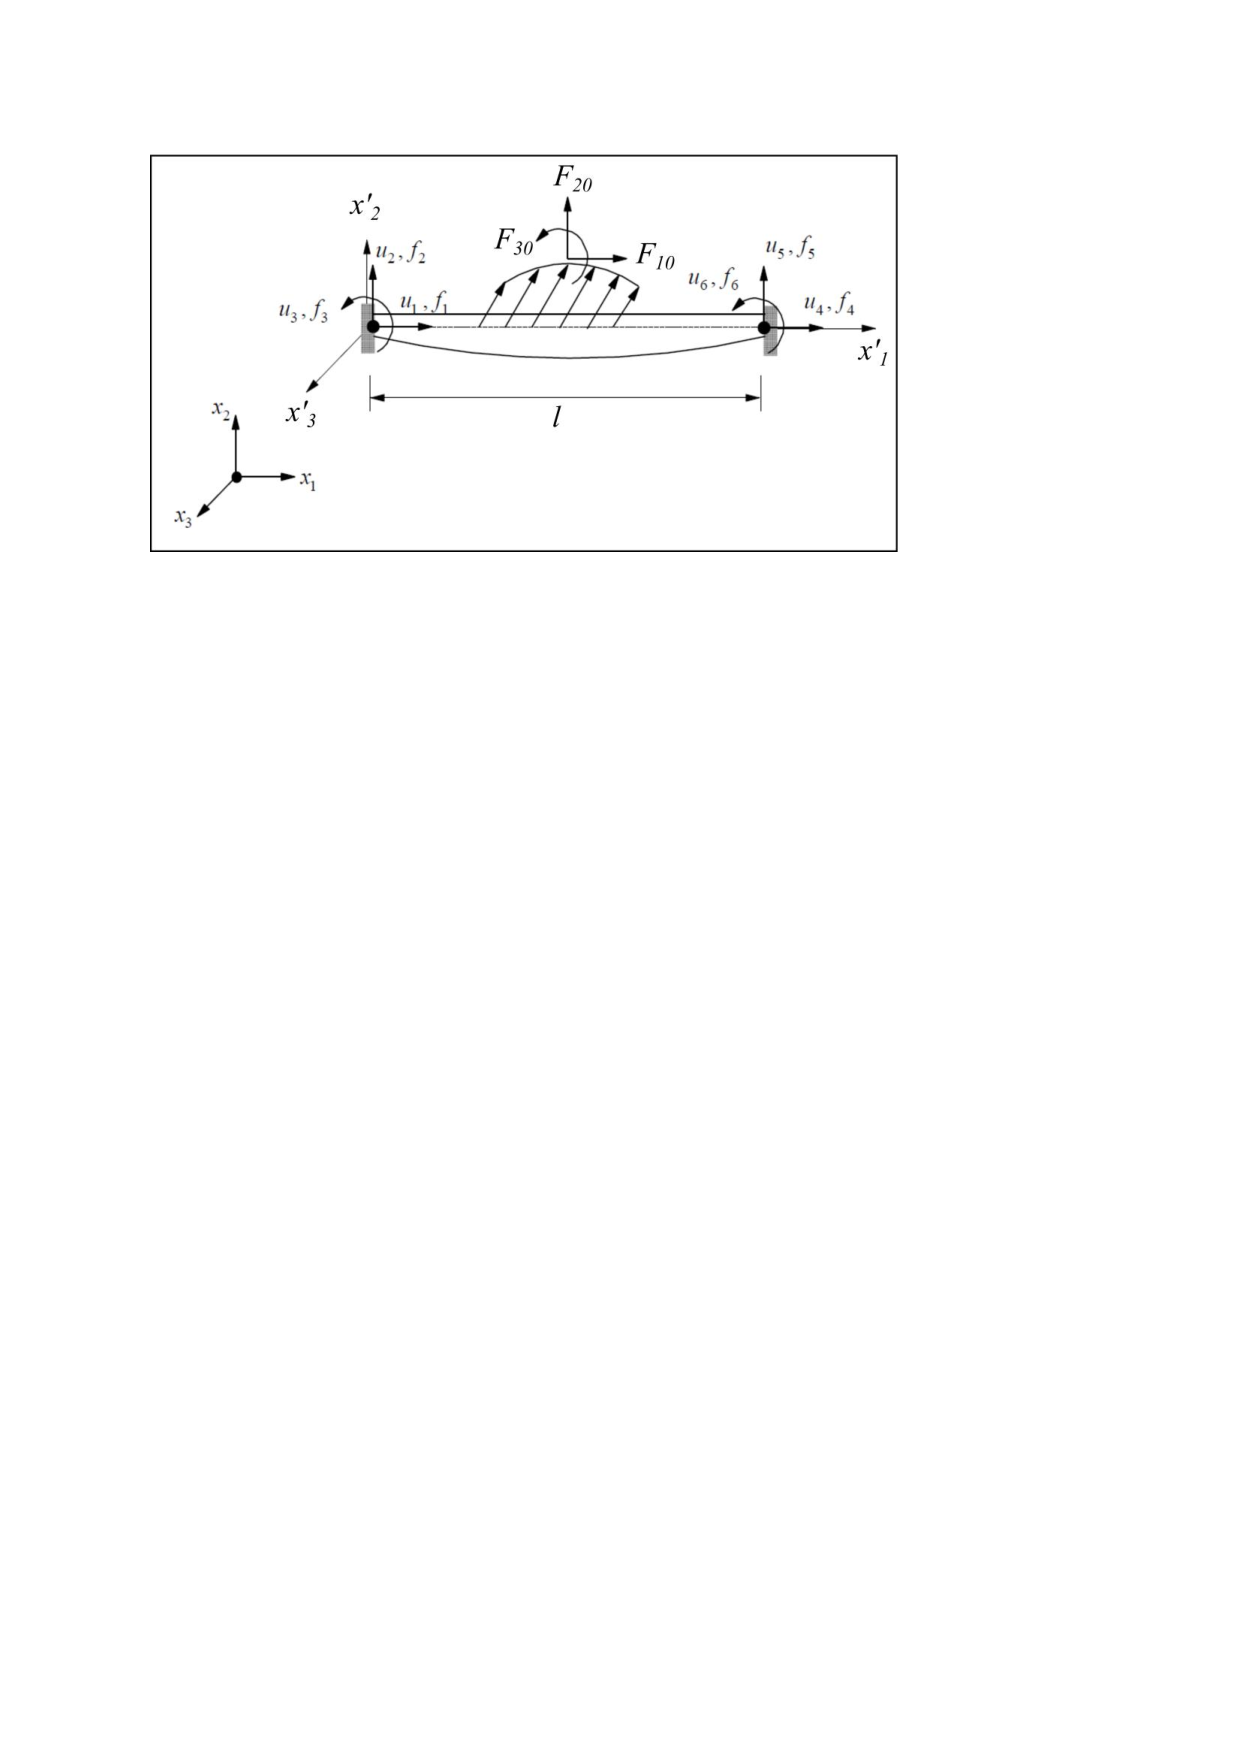
\includegraphics[trim = 27mm 205mm 59mm 27.5mm, clip, scale=1.2]{img/el-portico-plano.pdf}
	\caption{Elemento de Pórtico Plano}
	\label{fig:el-portico-plano}
\end{figure}

As equações de equilíbrio para este elemento são dadas por:

\begin{align}
	\label{eq:equilibrio}
	\sum F_{x'_1} & = f_1 + f_4 + F_{10} = 0 \nonumber \\
	\sum F_{x'_2} & = f_2 + f_5 + F_{20} = 0 \nonumber \\
	\sum F_{x'_3} & = f_3 + f_6 - f_2l + F_{30} = 0
\end{align}

onde $F_{i0}, i=1,2,3$ representa a ação resultante na direção $i$ devida à carga de membro, i.e.,

\begin{equation}
	\label{member_res}
	F_{10}=\int_{0}^{l}q_1(x'_1)dx'_1 \; ; \quad
	F_{20}=\int_{0}^{l}q_2(x'_1)dx'_1\; ;\quad
	F_{30}=\int_{0}^{l}\left[q_3(x'_1)-q_2(x'_1)(l-x_1)\right] dx'_1  \; ,
\end{equation}

\noindent em que as expressões de momento em (\ref{eq:equilibrio}) (última equação) e em (\ref{member_res}) ($F_{30}$) foram estabelecidas em relação à seção em $x_1=l$.

Aplicando-se o Princípio dos Forças Virtuais (PFV) e considerando-se o estado de carregamento mostrado na Fig. \ref{fig:estado-carregamento}, estabelece-se a seguinte equação de compatibilidade de deslocamentos:

\begin{align}
	\label{eq:PVF}
	\bar{f}_i u_{ij} & = \int_l \bar{M}_i \,d\beta_j + \int_l \bar{N}_i \,du_j + \int_l \bar{Q}_i \,dw_{sj},\quad i,j=1,\cdots,6.
\end{align}

onde $u_{ij}$ é o deslocamento nodal na direção do grau de liberdade $i$ devido à causa $j$, $\bar{M}_i$, $\bar{N}_i$ e $\bar{Q}_i$ são, respectivamente, o momento fletor, a força cortante e a força normal devidos a $\bar{f}_i=1$, ou seja,

\begin{align}
	\bar{M}_i = M(\bar{f}_i), \bar{N}_i = N(\bar{f}_i), \bar{Q}_i = Q(\bar{f}_i),
\end{align}

e $d\beta_j$, $du_j$ e $dw_{sj}$ denotam respectivamente a rotação flexional, o deslocamento axial e o deslizamento transversal (por cisalhamento) relativos, em uma seção $x'$ do elemento.

\begin{figure}[!htbp]
	\centering
	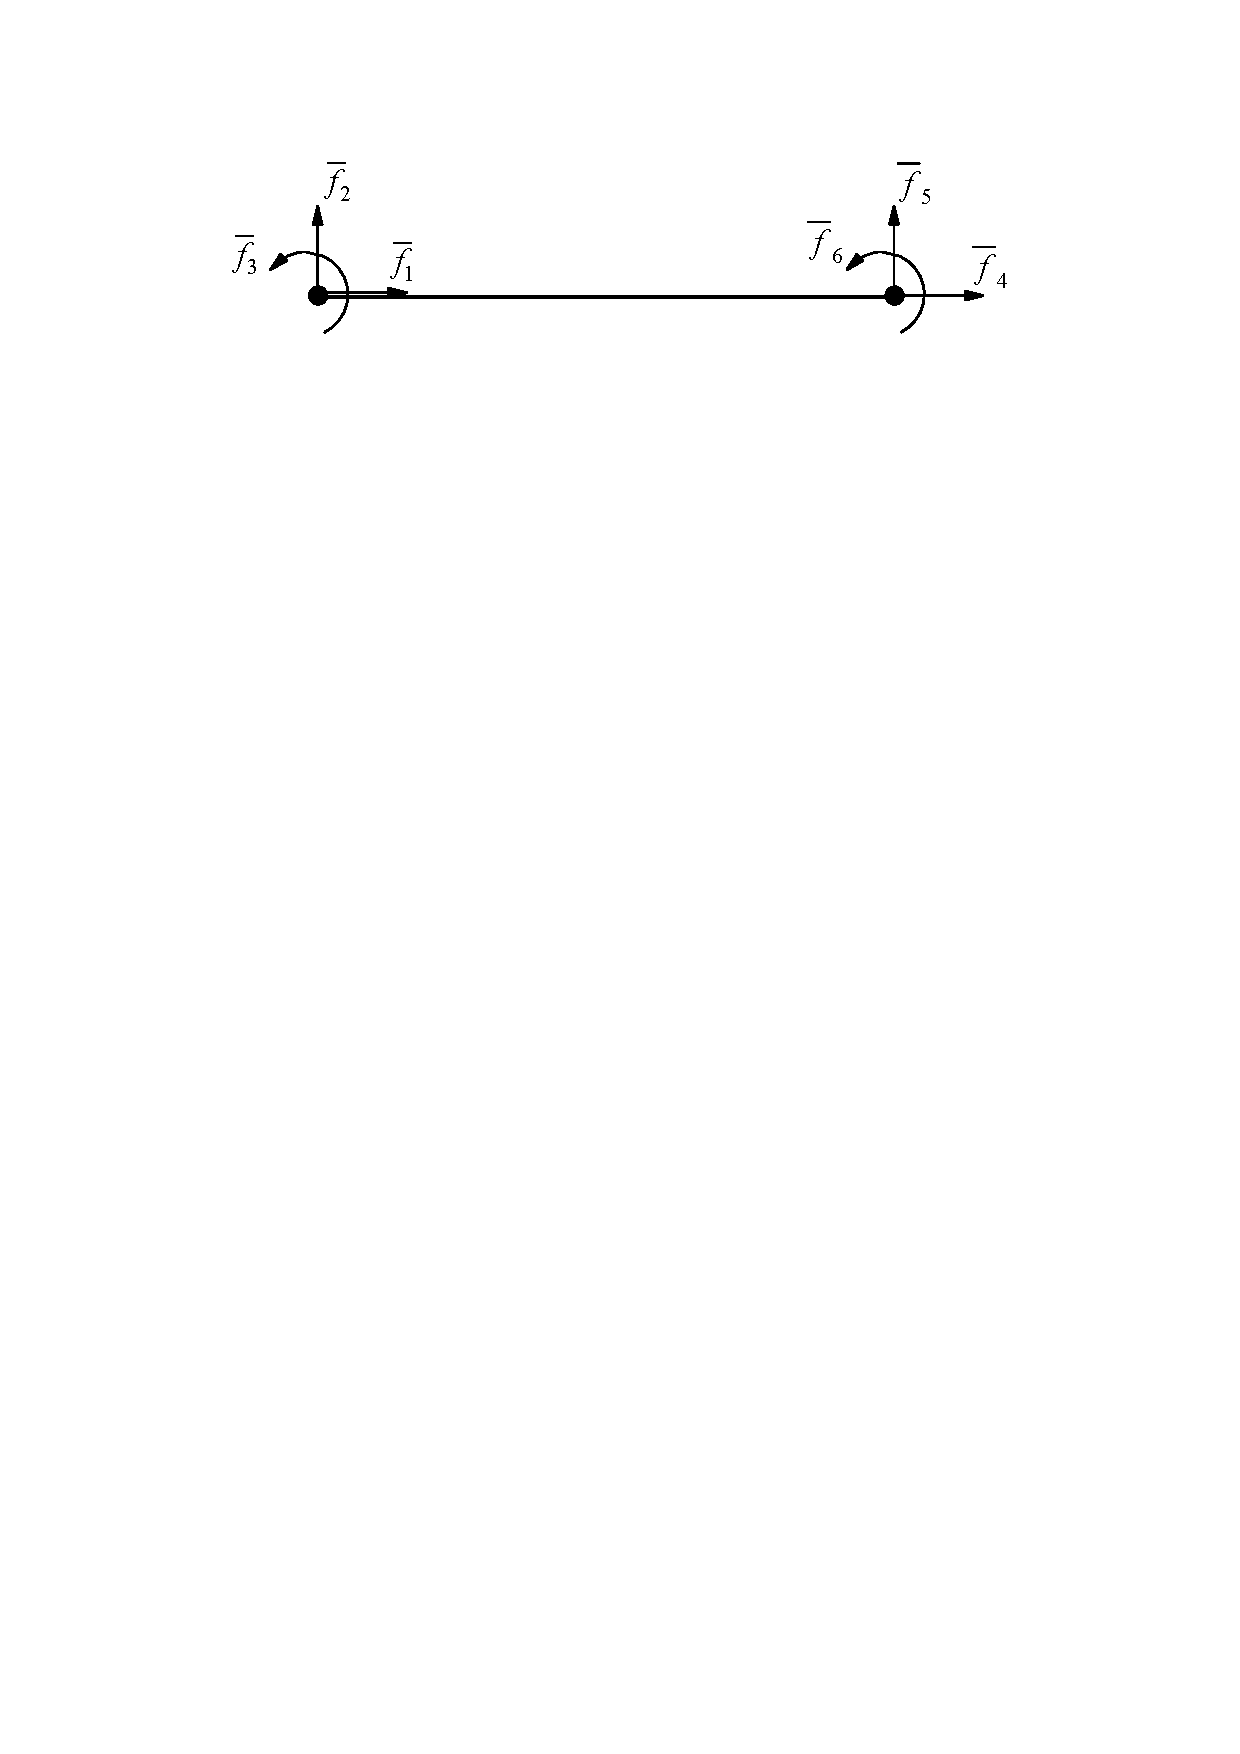
\includegraphics[trim = 30mm 240mm 40mm 25mm, clip, scale=.9]{img/estado-carregamento.pdf}
	\caption{Estado de Carregamento}
	\label{fig:estado-carregamento}
\end{figure}

Utilizando-se as equações \ref{eq:equilibrio} e \ref{eq:PVF}, podem então ser derivadas as expressões genéricas para rigidez de elemento e ações de engastamento nos casos mais gerais de características geométricas de elemento e de carregamentos. Para isso, consideram-se dois casos: em um deles o nó restringido é o inicial (nó esquerdo); no outro, o nó restringido é o nó final (nó direito, vide Fig. \ref{fig:casos-considerados})

\begin{figure}[!htbp]
	\centering
	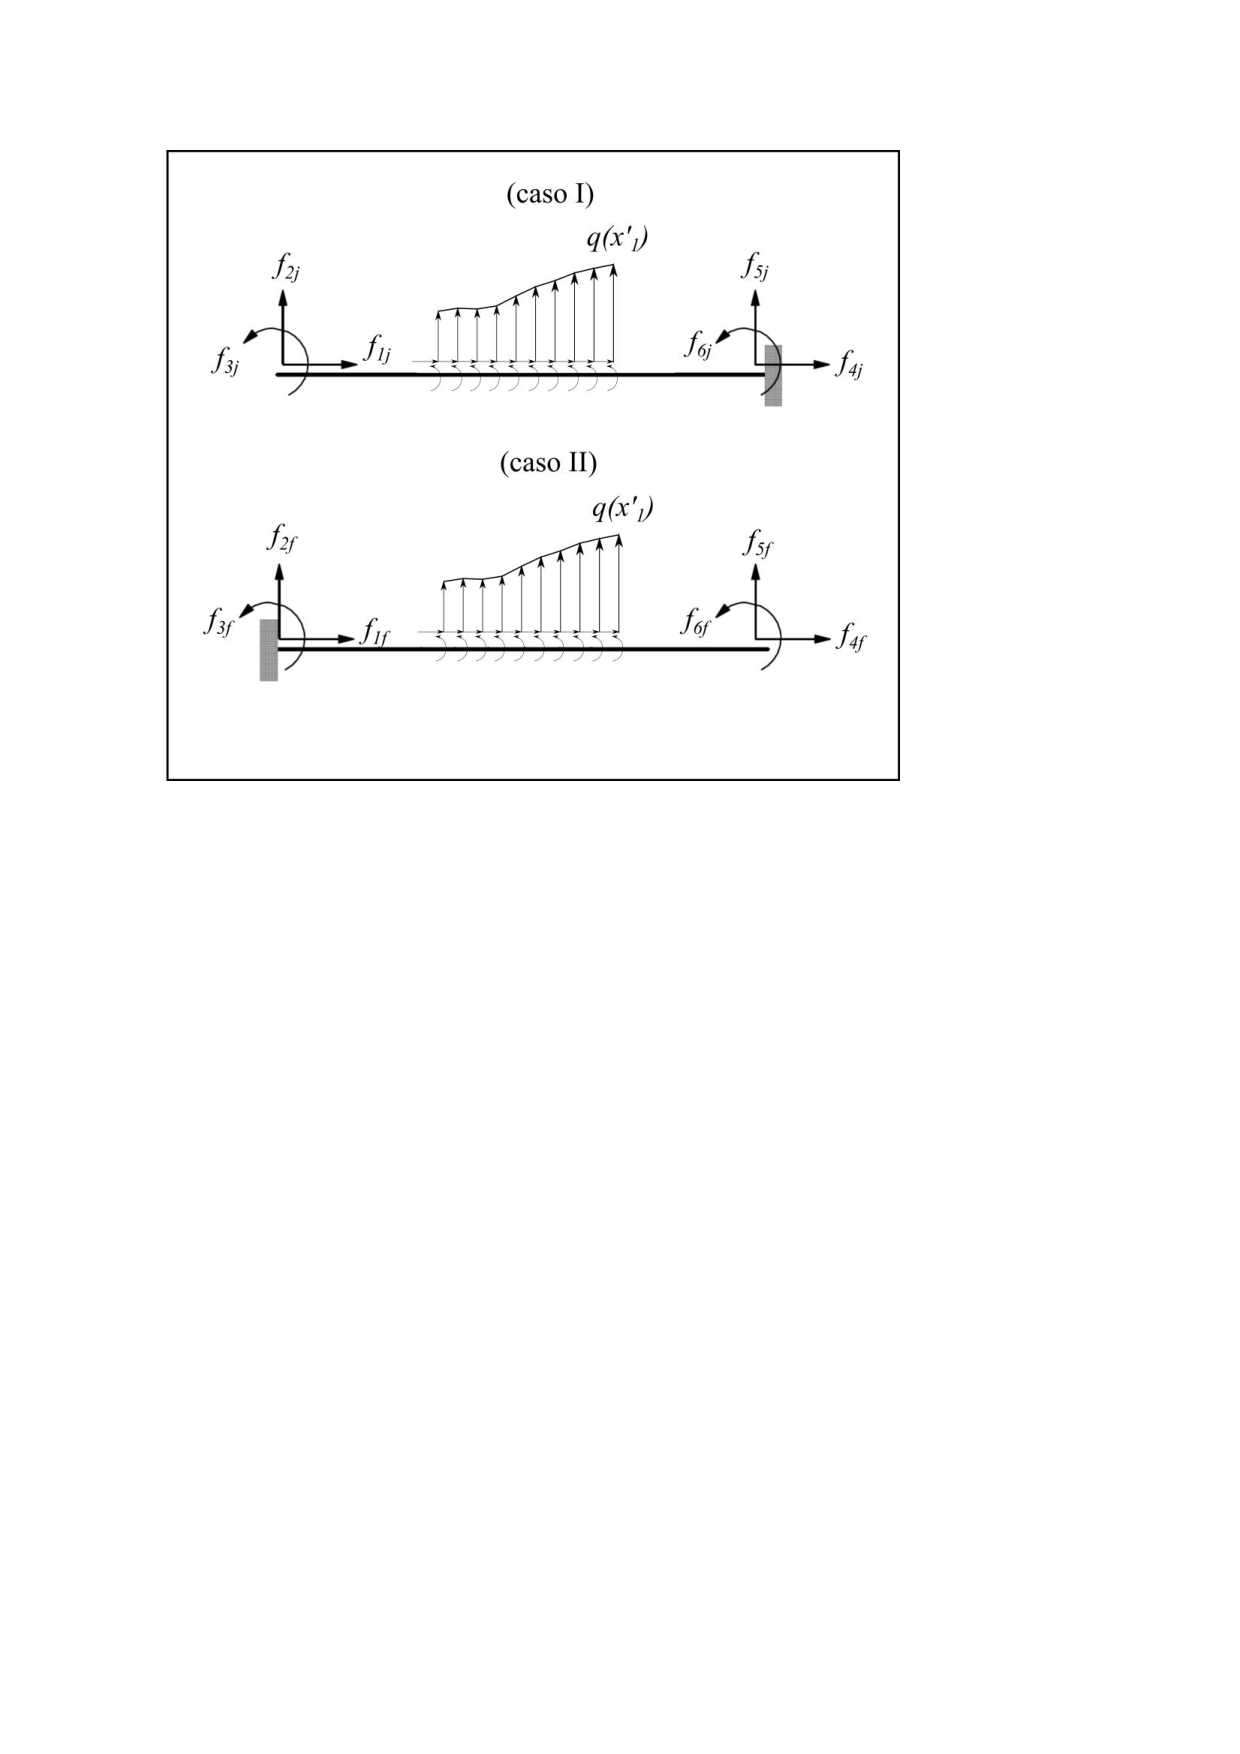
\includegraphics[trim = 30mm 180mm 60mm 30mm, clip, scale=1]{img/casos-considerados.pdf}
	\caption{Casos Considerados}
	\label{fig:casos-considerados}
\end{figure}

No caso I mostrado na Fig \ref{fig:casos-considerados}, tem-se $u_4=u_5=u_6=0$, e assim, as equações \ref{eq:equilibrio} e \ref{eq:PVF}, incluindo-se a influência do carregamento que atua no elemento, podem ser escritas como segue:

\begin{equation}
	\begin{bmatrix}
		\mathbf{E}_{II} & \mathbf{E}_{IF} \\
		\mathbf{A}_{II} & \mathbf{0}
	\end{bmatrix}
	\begin{bmatrix}
		\mathbf{f}_{Ii} \\
		\mathbf{f}_{Fi}
	\end{bmatrix}
	=
	\begin{bmatrix}
		-\mathbf{F}_0 \\
		\mathbf{u}_{Ii} - \mathbf{u}_{I0}
	\end{bmatrix}
	\label{eq:caso1-Aii}
\end{equation}

onde,

\begin{equation}
	\mathbf{E}_{II} =
	\begin{bmatrix}
		1 & 0  & 0 \\
		0 & 1  & 0 \\
		0 & -l & 1
	\end{bmatrix}
	, \;
	\mathbf{E}_{IF} =
	\begin{bmatrix}
		1 & 0 & 0 \\
		0 & 1 & 0 \\
		0 & 0 & 1
	\end{bmatrix}
	= \mathbf{I}_3.
\end{equation}

Note que, como se quer determinar as ações de extremidade de elemento tanto em consequência de deslocamentos prescritos segundo direção `j' como também em consequência do carregamento de elemento, $q(x)$, então a equação \ref{eq:PVF} será escrita na forma

\begin{equation}
	\bar{f}_i u_{ij}
	=
	\sum_{k=k_0}^{k_1} \int_l \dfrac{\bar{N}_i N_{kj}}{k_a(x)} \,dx
	+ \sum_{k=k_0}^{k_1} \int_l \dfrac{\bar{Q}_i Q_{kj}}{k_s(x)} \,dx
	+ \sum_{k=k_0}^{k_1} \int_l \dfrac{\bar{M}_i M_{kj}}{k_b(x)} \,dx
	+ u_{iq},
\end{equation}

em que `i' é o grau de liberdade onde se mede o efeito, e  `j' associa-se com a causa, e $u_{iq}$ denota deslocamento segundo grau de liberdade $i$ devido ao carregamento de elemento. Nesta equação,

\begin{equation}
	N_{kj} = N(f_{kj}),\quad Q_{kj} = Q(f_{kj}),\quad M_{kj} = M(f_{kj})
\end{equation}

e pode-se ainda escrever

\begin{equation}
	\bar{f}_i u_{ij}
	=
	\int_l \dfrac{\bar{N}_i  N_{j}}{k_a(x)} \,dx
	+ \int_l \dfrac{\bar{Q}_i Q_{j}}{k_s(x)} \,dx
	+ \int_l \dfrac{\bar{M}_i M_{j}}{k_b(x)} \,dx
	+ u_{iq},
\end{equation}

em que

\begin{equation}
	N_j =
	\sum_{k=k_0}^{k_1} N_{kj},\quad Q_j =
	\sum_{k=k_0}^{k_1} Q_{kj}, \quad M_j =
	\sum_{k=k_0}^{k_1} M_{kj}.
	\nonumber
\end{equation}

Acima,

\begin{align}
	i,j & = (m-1)\cdot ndofn + 1, m\cdot ndofn, \\ \nonumber
	m   & = 1,2,                                \\ \nonumber
	k_0 & = (m-1)\cdot ndofn +1,                \\ \nonumber
	k_1 & = m \cdot ndofn,
\end{align}

\begin{equation}
	\mathbf{f}_{Ii} =
	\begin{bmatrix}
		f_{1i} \\
		f_{2i} \\
		f_{3i}
	\end{bmatrix}, \;
	%% 
	\mathbf{f}_{Fi} =
	\begin{bmatrix}
		f_{4i} \\
		f_{5i} \\
		f_{6i}
	\end{bmatrix}, \;
	%%
	\mathbf{u}_{Ii} =
	\begin{bmatrix}
		u_{1i} \\
		u_{2i} \\
		u_{3i}
	\end{bmatrix} =
	\begin{bmatrix}
		\delta_{1i} \\
		\delta_{2i} \\
		\delta_{3i}
	\end{bmatrix}, \;
\end{equation}

onde $\delta_{ki}$ é o delta de Kronecker, e

\begin{align}
	u_{iq}
	 & =\sum_{k=1}^3 \left( \int_l \dfrac{\bar{M}_i\,\, ^{(m)}M_{kq}}{k_b} dx'_1 + \int_l \dfrac{\bar{N}_i\,\, ^{(m)}N_{kq}}{k_a} dx'_1 + \int_l \dfrac{\bar{Q}_i\,\, ^{(m)}Q_{kq}}{k_s} dx'_1 \right) \\
	 & = \int_l \dfrac{\bar{M}_i\,\, ^{(m)}M_{q}}{k_b} dx'_1 + \int_l \dfrac{\bar{N}_i\,\, ^{(m)}N_{q}}{k_a} dx'_1 + \int_l \dfrac{\bar{Q}_i\,\, ^{(m)}Q_{q}}{k_s} dx'_1 ,
	\; i=1,2,3,\,\,\,
\end{align}

em que

\begin{align}
	M_{q} & =\sum_{k=1}^3 {^{(m)}M_{kq}},\quad N_{q}=\sum_{k=1}^3 {^{(m)}N_{kq}},\quad Q_{q}=\sum_{k=1}^3  {^{(m)}Q_{kq}}, \\   \nonumber
	                                                                                                                            ^{(m)}M_{kq}&= M(q_k),\,\, ^{(m)}N_{kq} = N(q_k),\,\, ^{(m)}Q_{kq} = Q(q_k).
\end{align}

Nessas expressões, $k_b=EI$, $k_a=EA$ e $k_s=\dfrac{GA}{\chi}$ denotam, respectivamente, as rigidezes de seção flexional, axial e ao cisalhamento.

Os coeficientes de $\mathbf{A}_{II}$ resultam da equação

\begin{equation}
	\int_l \dfrac{\bar{M}_i M_{j}}{k_b} dx'_1 + \int_l \dfrac{\bar{N}_i N_{j}}{k_a} dx'_1 + \int_l \dfrac{\bar{Q}_i Q_{j}}{k_s} dx'_1  = \sum_{m=1}^3 a_{im} f_{mj} = u_{ij} - u_{iq},
	\quad
	i,j = 1,2,3.
	\label{eq:Aii}
\end{equation}

em que as ações $f_{kj}$ envolvidas nas funções $M_j$, $N_j$ e $Q_j$
foram isoladas. O termo $\chi$ usado na definição de $k_s$ é o fator de forma da seção para o cisalhamento (em relação à direção $x'_2$) dado por

\begin{equation}
	\chi = \dfrac{A}{I_{x_2}^2} \int_{y_b}^{y_t} \dfrac{M_s^2(x'_2)}{b(x'_2)} dx'_2,
\end{equation}

onde $M_s^2(x'_2)$ é o momento estático da porção de área acima da reta $x'_2$, dado por

\begin{equation}
	M_s^2(x'_2) = \int_{y}^{y_t} \eta b(\eta)\,d\eta,
\end{equation}

sendo $y$ a ordenada do ponto onde se calcula a tensão cisalhante, e $y_b$ e $y_t$, respectivamente as ordenadas dos pontos-limites inferior e superior da seção. Em geral, define-se a rigidez ao cisalhamento, $k_s$, da seção transversal do elemento por

\begin{equation}
	k_s=GA_{s} = \dfrac{GA}{\chi} \; ,
\end{equation}

\noindent em que $A_s$ é a área efetiva de cisalhamento. Na tabela abaixo, indicam-se as expressões para o cálculo de $A_s$ para seções usuais e para uma seção genérica.

\begin{figure}[!htbp]
	\centering
	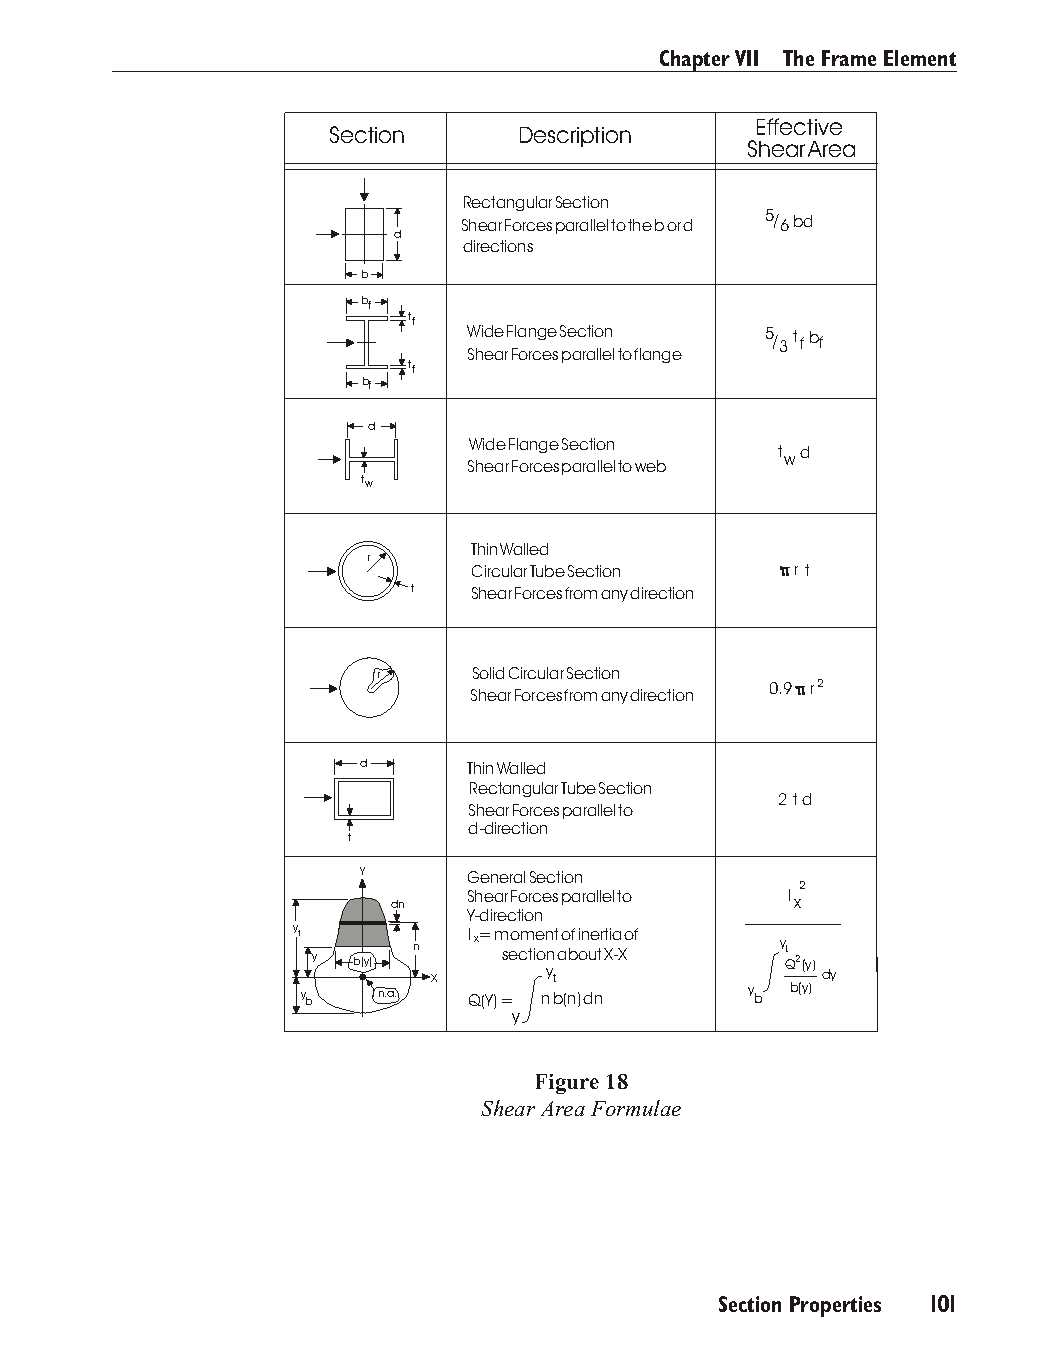
\includegraphics[trim = 4.5cm 5cm 2cm 1.5cm, clip, scale=1]{img/sap-2000.pdf}
	\caption{Áreas efetivas de cisalhamento (vide \textit{Analysis Reference Manual for the SAP2000})}
	\label{fig:sap-2000}
\end{figure}

Para o segundo caso ($m=2$), com $u_1 = u_2 = u_3 = 0$, figura~\ref{fig:casos-considerados}, expressões semelhantes às mostradas em ~\ref{eq:caso1-Aii} podem ser obtidas. Tem-se:

\begin{equation}
	\begin{bmatrix}
		\mathbf{E}_{II} & \mathbf{E}_{IF} \\
		\mathbf{0}      & \mathbf{A}_{FF} \\
	\end{bmatrix}
	\begin{bmatrix}
		\mathbf{f}_{If} \\
		\mathbf{f}_{Ff}
	\end{bmatrix}
	=
	\begin{bmatrix}
		-\mathbf{F}_0 \\
		\mathbf{u}_{Ff} - \mathbf{u}_{F0}
	\end{bmatrix},
	\label{eq:caso2-Aff}
\end{equation}

onde

\begin{equation}
	\mathbf{f}_{If} =
	\begin{bmatrix}
		f_{1f} \\
		f_{2f} \\
		f_{3f} \\
	\end{bmatrix}, \qquad
	%% 
	\mathbf{f}_{Ff} =
	\begin{bmatrix}
		f_{4f} \\
		f_{5f} \\
		f_{6f} \\
	\end{bmatrix}, \qquad
	%%
	\mathbf{u}_{If} =
	\begin{bmatrix}
		u_{4f} \\
		u_{5f} \\
		u_{6f} \\
	\end{bmatrix} =
	\begin{bmatrix}
		\delta_{4f} \\
		\delta_{5f} \\
		\delta_{6f} \\
	\end{bmatrix}, \quad
	f=4,5,6,
\end{equation}

onde $\delta_{kf}$ é o delta de Kronecker, e

\begin{align}
	u_{iq}
	 & = \sum_{k=4}^6 \left(
	\int_l \dfrac{\bar{M}_i\,\, ^{(m)}M_{kq}}{k_b} dx'_1 +
	\int_l \dfrac{\bar{N}_i\,\, ^{(m)}N_{kq}}{k_a} dx'_1 +
	\int_l \dfrac{\bar{Q}_i\,\, ^{(m)}Q_{kq}}{k_s} dx'_1 \right)                                                                                                               \\
	 & = \int_l \dfrac{\bar{M}_i\,\, ^{(m)}M_{q}}{k_b} dx'_1 + \int_l \dfrac{\bar{N}_i\,\, ^{(m)}N_{q}}{k_a} dx'_1 + \int_l \dfrac{\bar{Q}_i\,\, ^{(m)}Q_{q}}{k_s} dx'_1 \quad
	i=4,5,6,
\end{align}

em que

\begin{align}
	M_{q}
	 & =\sum_{k=4}^6 {^{(m)}M_{kq}},\quad N_{q}=\sum_{k=4}^6 {^{(m)}N_{kq}},\quad Q_{q}=\sum_{k=4}^6  {^{(m)}Q_{kq}}, \\   \nonumber
	                                                                                                                       ^{(m)}M_{kq}
	 & = M(q_k),\,\, ^{(m)}N_{kq} = N(q_k),\,\, ^{(m)}Q_{kq} = Q(q_k).
\end{align}
A matriz $\mathbf{A}_{FF}$ é dada pela equação \ref{eq:Aii} para $i,j=4,5,6$.
